%==============================================================================
%== template for LATEX poster =================================================
%==============================================================================
%
%--A0 beamer slide-------------------------------------------------------------
\documentclass[5pt, final]{beamer}
\usepackage[orientation=portrait, size=a0,
            scale=1.25         % font scale factor
           ]{beamerposter}
           
\geometry{
  hmargin=2.5cm, % little modification of margins
}

%
\usepackage[utf8]{inputenc}

\linespread{1.05}
%
%==The poster style============================================================
\usetheme{sharelatex}

%==Title, date and authors of the poster=======================================
\title
[Agile Vorgehensmodelle, Master, WS 202425] % Conference
{ % Poster title
	Die Rolle des Scrum Masters: Moderation, Konfliktlösung und Teamförderung
}

\author{ % Authors
	Nico Riedlinger\inst{1}, Marc Weiss\inst{1}
}
\institute
[Very Large University] % General University
{
	\inst{1} HTWG Konstanz
}
\date{\today}



\begin{document}
	\begin{frame}[t]
		%==============================================================================
		\begin{multicols}{3}
			%==============================================================================
			%==The poster content==========================================================
			%==============================================================================
			
			\section{Aufgabenbereich}
			
%			In Ref.~\cite{ref1}...
%			In Refs.~\cite{ref1,ref2}...
%			On webpage~\cite{web}...
			Der Aufgabenbereich eines Scrum Masters ist sehr vielseitig.
			Als Teil des Teams übernimmt er eine koordinierende Rolle und ist Ansprechpartner in Problemsituationen \cite{meindl12}.
			Diese können bezogen auf die technische Seite, zum Beispiel mit dem zu entwickelnden Produkt, oder auf sozialer Ebene sein.
			Bei Unstimmigkeiten im Team ist der Scrum Master dafür verantwortlich, diese Konflikte zu beseitigen.
			
			Eine Einordnung des Scrum Masters innerhalb des Teams ist in Figure \ref{fig:sm-team} zu sehen.
			Hier bildet er eine Schnittstelle vom Team nach außen gegenüber Managern.
			
			\vskip1ex
			\begin{figure}
				\centering
				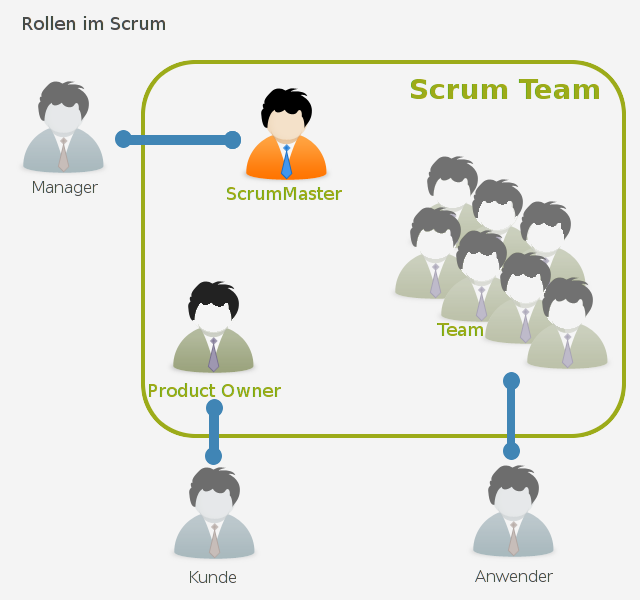
\includegraphics[width=0.95\columnwidth]{scrummaster}
				\caption{Einordnung des Scrum Masters innerhalb des gesamten Teams. Quelle: \cite{meindl12}}\label{fig:sm-team}
			\end{figure}
			\vskip2ex
			
			Des Weiteren ist er für die Organisation und Moderation von Besprechungen im Scrum-Kontext zuständig.
			Das umfasst sowohl das Sprint Planning als auch die Sprint Review sowie Retrospektive (kurz: Retro).
			Er verteilt im Voraus die jeweilige Agenda und moderiert die einzelnen Besprechungen.
			Letzteres gilt außerdem für das Daily Scrum.
			
			\subsection{Konfliktlösung}
			
			Ein weiterer wesentlicher Aspekt der Rolle des Scrum Masters ist die Konfliktlösung. Scrum Masters sind oft in der Lage, Konflikte innerhalb des Teams zu erkennen und zu lösen, indem sie als neutrale Vermittler agieren. Dies ist besonders wichtig, da Konflikte die Teamleistung negativ beeinflussen können \cite{Noll17}.
			
			\subsection{Moderation}
			
			Der Scrum Master moderiert die Besprechungen, um eine hohe Effektivität in der Teamkommunikation und das Erreichen der Ziele sicherzustellen \cite{vantighem24}.
			Unter korrektem Einsatz verschiedener Techniken kann die Qualität von Besprechungen wie auch die Motivation der Teilnehmer für eine solche Besprechung erheblich gesteigert werden.
			
			Eine der Techniken ist die Erstellung und Überprüfung von Teamregeln.
			Ähnlich wie die \textit{Definition of Done} oder \textit{Definition of Ready} für das Erstellen und Abschließen von User Storys, handelt es sich hierbei um einen dynamischen Regelsatz.
			Dieser kann je nach Aufgaben und Anforderungen des Teams in gemeinsamer Absprache angepasst werden.
			Der Scrum Master beobachtet das Team während Besprechungen und weist, ähnlich wie ein Schiedsrichter, auf Verstöße gegen die Regeln hin.
			Bei zu vielen Verstößen muss ein Grund dafür mit dem gesamten Team gefunden und gegebenenfalls das Regelwerk angepasst werden.
			
			% Moderation unabhängig von Führungsrolle durchführen, um Interessenskonflikte zu vermeiden.
            Weitere Techniken für eine gute Besprechungsqualität sind Timeboxing und neutrale Moderation \cite[S. 23ff.]{malten24}.
            Beim Timeboxing geht es darum, die vorab kommunizierten Zeiten für eine Besprechung einzuhalten.
            Sowohl der Anfangszeitpunkt als auch das Ende sollten nicht überzogen werden.
            Wenn es dennoch mehr Gesprächsbedarf als verfügbare Zeit geben sollte, muss der Scrum Master als Moderator eine geeignete Lösung finden, ohne die Timebox zu überziehen.
            Als Beispiele dafür seien ein zusätzlicher Termin, persönliches Gespräch unter den Beteiligten oder eine Vertagung auf den nächsten regulären Besprechungstermin genannt.
            
			In der Praxis umfasst die Rolle des Scrum Masters auch Aktivitäten wie das \textit{Facilitating} (erleichtern, vorplanen), Mentoring und Koordinieren, um die Teamarbeit zu unterstützen und Hindernisse zu beseitigen.
            Diese Moderationsfähigkeiten sind besonders wichtig, um sicherzustellen, dass das Team die Scrum-Praktiken regelmäßig und effektiv umsetzt \cite{Shastri21}.
			
			\subsection{Teamförderung}
			
			Die Förderung des Teams ist ein zentraler Bestandteil der Rolle des Scrum Masters.
            Dies beinhaltet die Unterstützung des Teams bei der Selbstorganisation und Übernahme von Führungsrollen, während das Team reift \cite{?}.
            Scrum Masters tragen zur Dynamik und zum Wohlbefinden des Teams bei, indem sie das Team herausfordern, seine Leistung zu steigern und Wissen zu teilen \cite{?}.
            Die Förderung eines unterstützenden internen Teamklimas ist entscheidend für den Erfolg des Scrum Masters in dieser Rolle \cite{?}.
            
            Als Technik zur Teamförderung können agile Spiele eingesetzt werden.
            In \cite{bless24} sind viele verschiedene aufgeführt.
            Sie lassen sich in mehrere Kategorien unterteilen, so zum Beispiel Teambuilding/Teamwork, Selbstorganisation oder Multitasking.
            Solche Spiele können sowohl in neu zusammengefundenen Teams zum Kennenlernen als auch in bereits länger bestehenden Teams zur Festigung oder Verbesserung des Scrum-Prozesses eingesetzt werden.
            Üblicherweise nutzen sie das Teambuilding oder eine Komponente von Scrum auf einer höheren Abstraktionsebene aus und verwenden viele Metaphern.
            Ein Spiel, was besonders das iterative und inkrementelle Vorgehen von Scrum vermittelt, ist die \textit{Marshmallow Challenge}.
            Es geht darum, einen höchstmöglichen Turm aus rohen Spaghetti zu bauen und auf der Spitze ein Marshmallow zu platzieren.
            Die Entwürfe der Teams werden in der Regel mehrfach überarbeitet und ausgebaut bis das finale Produkt steht.
			
			\section {Führungsverhalten}
            
            //hier fehlen noch ein paar einleitende Sätze
            
            \subsection{Servant Leadership}
			
			//noch nicht so gut formuliert der Part...
			
			Ein Servant Leader ist eine Führungsperson, die nicht beherrschend auf ihr Team einwirkt, sondern dienend führt.
            Dies beschreibt den Scrum Master, der speziell zu Beginn eines neuen Teams zwar eine Führungspersönlichkeit, die dem Team dient, darstellt, aber dennoch das Team wichtige Entscheidungen treffen lässt.
            Die Fähigkeit, Konflikte zu managen, wird auch durch die Anwendung von \textit{Servant Leadership} unterstützt, was die Effektivität des Teams steigern kann.
			„Die wichtigsten Einflussfaktoren für erfolgreiches Führungsverhalten sind die technischen, organisatorischen und kommunikativen Kompetenzen der Scrum Master. Darüber hinaus sind Selbstorganisation, Wissensmanagement sowohl Einflussfaktor als auch Kennzeichen erfolgreichen Führungsverhaltens.“ …
            Empowering-Leadership-Theorie: So wird die positive Wirkung von Empowerment auf die Arbeitsleistung und das Commitment… Einfluss der Beziehung zwischen Scrum Mastern und Teammitgliedern auf den Führungserfolg und auf die Team effektivität [6]
			
			\subsection{Abgrenzung zum Product Owner}
			
			% Scrum Master vs. Product Owner
            Die Rollen des Scrum Masters und Product Owners werden oftmals miteinander vermischt, teilweise sogar von der gleichen Person ausgeführt.
            Dabei haben beide Rollen sehr unterschiedliche Verantwortlichkeiten und Charakteristiken \cite{sutherland14}.
            
            % kurzer Abriss von PO
            Diese Unterschiede sind bereits in Figure \ref{fig:sm-team} zu sehen.
            Während sich der Scrum Master um das Team kümmert und versucht, mögliche Blockaden zu beseitigen, ist der Product Owner am entstehenden Produkt interessiert \cite{Spiegler21}.
%            Er steht in konstantem Austausch zu den Kunden, nimmt deren Anforderungen auf und diskutiert diese.
%            Anschließend zerkleinert der Product Owner die Anforderungen in einzelne Teile und formuliert sie als User Story.
%            Auf Basis dieser User Storys kann er nun dem Entwicklungsteam das weitere Vorgehen präsentieren.
            Er ist aus Sicht des Kunden verantwortlich.
            Außerdem kommuniziert er dem Entwicklungsteam das weitere Vorgehen.
            
            % eine Person, zwei Rollen = Interessenskonflikte
            Aufgrund der unterschiedlichen Aufgabenbereiche kann es zu Interessenskonflikten kommen, wenn die Rollen des Scrum Masters und des Product Owners von der gleichen Person ausgeführt werden.
%            Da der Scrum Master eigentlich für die Probleme des Teams und die Beseitigung derer zuständig ist, fungiert er auch als eine Art \textit{Vertrauensperson} in Problemfällen.
            Der Scrum Master bildet eine Art \textit{Vertrauensperson} bei Problemen gegenüber dem Team.
            Diese Vertrauensperson steht dem Team allerdings nicht zur Verfügung, wenn sie gleichzeitig für den Erfolg des Produkts verantwortlich ist \cite{me-company}.
            Sieht sie diesen in Gefahr, wird sie höchstwahrscheinlich auch dementsprechend handeln.
            Dadurch entsteht ein Misstrauen gegenüber des Scrum Masters bzw. Product Owners.
%            Die Teammitglieder können sich nicht mehr mit ihren Problemen an die Vertrauensperson wenden.
            Infolgedessen werden Probleme nie behoben und im schlimmsten Fall zerfällt das Team.
			
			\section{Ergebnisse}
			
            \begin{itemize}
    			\item Steigerung der Produktivität des Teams \cite{vantighem24}.
    			\item Abschirmung nach Außen vor zum Beispiel Management und Organisation der Anforderungen mit dem PO \cite{meindl12}.
                \item Nicht autom. twice as much in half as much time nur wegen Einführung Scrum \cite{sutherland14}.
                \item Klare Rollentrennung zwischen Scrum Master und Product Owner.
            \end{itemize}
			
%			\vskip1ex
%			\begin{table}
%				\centering
%				\caption{This is a table with scientific results.}
%				\begin{tabular}{ccccc}
%					\hline\hline
%					1 & 2 & 3 & 4 & 5\\
%					\hline
%					aaa & bbb & ccc & ddd & eee\\
%					aaaa & bbbb & cccc & dddd & eeee\\
%					aaaaa & bbbbb & ccccc & ddddd & eeeee\\
%					aaaaaa & bbbbbb & cccccc & dddddd & eeeeee\\
%					1.000 & 2.000 & 3.000 & 4.000 & 5.000\\
%					\hline\hline
%				\end{tabular}
%			\end{table}
%			\vskip2ex
			
			%==============================================================================
			%==End of content==============================================================
			%==============================================================================
			
			%--References------------------------------------------------------------------
			
			\subsection{References}
						
			\begin{thebibliography}{99}
				
%				\bibitem{ref1} J.~Doe, Article name, \textit{Phys. Rev. Lett.}
%				
%				\bibitem{ref2} J.~Doe, J.~Smith, Other article name, \textit{Phys. Rev. Lett.}
%				
%				\bibitem{web} \url{http://www.google.pl}
				
				\bibitem{malten24} M.~Malten, Effektive Team-Meetings: Impulse aus der agilen Praxis für bessere Besprechungen und Kommunikation (2024). 1. Auflage. \textit{Springer Gabler Berlin, Heidelberg}. ISBN: 978-3-662-69816-7.
				
				\bibitem{meindl12} C.~Meindl, Der ScrumMaster, \url{https://alphanodes.com/de/der-scrummaster} (zul. besucht am 10.12.2024)
				
				\bibitem{me-company} Me~\&~Company~GmbH, Scrum Master: Coach, Moderator und Unterstützer, \url{https://www.me-company.de/magazin/scrum-master/} (zul. besucht am 10.12.2024)
				
				\bibitem{vantighem24} C.~Vantighem, Der Scrum Master: Definition, Aufgaben und Nutzen, \url{https://www.teammeter.com/de/scrum-master-aufgaben-verantwortung-und-nutzen} (zul. besucht am 10.12.2024)
				
				\bibitem{Shastri21} Y.~Shastri, R.~Hoda, R.~Amor (2021). Spearheading agile: the role of the scrum master in agile projects. Empirical Software Engineering. 26. Auflage.
				
				\bibitem{Noll17} J.~Noll, M.~Razzak, J~Bass, S.~Beecham (2017). A Study of the Scrum Master's Role. S. 307-323.
				
				\bibitem{Spiegler21} S.~Spiegler, C.~Heinecke, S.~Wagner (2021). An empirical study on changing leadership in agile teams. Empirical Software Engineering. 26. Auflage.
				
%				\bibitem{Kristensen21} S.~Kristensen, M.~Paasivaara (2021). What Added Value Does a Scrum Master Bring to the Organisation? — A Case Study at Nordea. 47th Euromicro Conference on Software Engineering and Advanced Applications (SEAA), S. 270-278.
				
%				\bibitem{Frye24} M.~Frye, H.~Möltner (2024). Selbstorganisiert und dennoch geführt – eine explorative Studie zur Führung durch Scrum Master.
                
                \bibitem{sutherland14} J.~Sutherland, JJ~Sutherland, Scrum: The Art of Doing Twice the Work in Half the Time (2014). \textit{Crown Currency}. ISBN: 978-0-385-34645-0.
                
                \bibitem{bless24} M.~Bleß, D.~Wagner, Agile Spiele - kurz \& gut (2024). 2. Auflage. \textit{O'Reilly Verlag GmbH \& Co. KG}. ISBN: 978-3-960-09249-0.
				
			\end{thebibliography}
			%--End of references-----------------------------------------------------------
			
		\end{multicols}
		
		%==============================================================================
	\end{frame}
\end{document}
